\let\textcircled=\pgftextcircled
\chapter{The LHC and the CMS experiment}
\label{chap:detector}

\initial{T}his chapter concerns the experimental setup. \acrshort{cern} is the organisation that manages the machines discussed and is a pioneer in the high energy physics community. As such, it will be given a short overview. The \acrlong{lhc} provides the \acrshort{cms} experiment with proton-proton collision data that is then stored, corrected, and then used by physicists for analyses. Ranging from \acrlong{sm} precision measurements, searches for new physics, the development of tools and algorithms to aid the previous two, these and much more are studied by the collaboration. \acrshort{cms} is described in detail, from its hardware and subdetectors to its data acquisition and trigger system. Special attention is given to the derivation of \acrfull{jec} in the \acrfull{l1t} as I have been a part of that effort during my PhD.

\begin{easylist}[itemize]
\ListProperties(Style*=-- , FinalMark={)}, Margin=0.5cm)
& Emphasise the jet and energy sum triggers in \acrlong{l1t} as I've worked on them, and Calorimeter Layer-2 for the same reason. Tie into SVJ and Hinv since they're hadronic searches.
\end{easylist}


%=========================================================


\section{CERN}
\label{sec:detector_cern}

\acrshort{cern}, the European Organisation for Nuclear Research (\emph{Organisation Europ\'{e}enne pour la Recherche Nucl\'{e}aire}), is the body responsible for large scale particle and high energy physics projects in Europe. It was founded in 1954 under the \emph{Conseil Europ\'{e}en pour la Recherche Nucl\'{e}aire} (European Council for Nuclear Research), from where its acronym derived. \acrshort{cern}'s primary site is situated in the canton of Geneva and creeps over the Franco-Swiss border. Its main purpose today is to provide physical and technological infrastructure for particle and high energy physics experiments. From large scale accelerators to extensive computing farms, \acrshort{cern} has grown into the largest laboratory for particle physics in the world. The organisation also provides a central community for the many researchers, engineers, and technicians to share ideas and collaborate effectively.

The organisation was founded by twelve European member states, the United Kingdom being one of them. It has since expanded to twenty three, encompassing most of western Europe and some of the continent's east. Many more countries from across the globe are affiliated with \acrshort{cern} in some way, providing researchers, computing resources, and more. The member states and associated members contribute to \acrshort{cern}'s budget, to the tune of 1.2 billion Swiss Francs for the year 2020 \cite{cern_budget_2020}.

Many important inventions and discoveries can be attributed to \acrshort{cern} and its personnel. Physics [achievements] include observations of weak neutral current interactions in 1973~\cite{HASERT1973121,HASERT1973138}, paving the way for the \PW~\cite{ARNISON1983103,BANNER1983476} and \PZ~\cite{Arnison:1983mk,Bagnaia:1983zx} boson discoveries with the UA1 and UA2 experiments in 1983. The number of light neutrino generations at the \acrfull{lep} in 1989~\cite{Trentadue:200667}, and direct CP violation with the NA48 experiment in 1999~\cite{Fanti_1999}, were also observed. Tim Berners-Lee and Robert Cailliau are credited with inventing the World Wide Web --- the ubiquitous service for accessing the internet --- in 1989/90.

\acrshort{cern} is perhaps most widely known as the home of the \acrlong{lhc}, the particle accelerator involved in the discovery of the Higgs boson~\cite{Chatrchyan:2012xdj,Aad:2012tfa}. More is discussed in Chpt.~\ref{sec:detector_lhc}. But \acrshort{cern} is still involved in many more undertakings. There are many fixed target experiments that use beams from the \acrshort{ps} and \acrshort{sps} such as COMPASS (studies hadronic structure) and NA62, investigating rare decays of kaons. Experiments like ALPHA and \acrshort{aegis} use antiprotons from the Antiproton Decelerator to study antimatter in detail. The \acrshort{isolde} facility at \acrshort{cern} delivers beams of radioactive ions to perform many nuclear physics experiments.

Concern is given not just to contemporary science, but also to the physics of tomorrow. The experiments and accelerators are frequently upgraded, for example \acrshort{lhc} improvements documented in Chpt.~\ref{subsec:evolution_lhc}. Future accelerators are also being discussed, such as the \acrfull{fcc}. The collider would use the \acrshort{lhc} as a booster, with the final ring having a 90--100\,km circumference and up to 100\TeV centre of mass energy. Proposals for the injectants are electron-positron beams (\acrshort{fcc}-ee, $\sqrt{s} = \text{90--350}\GeV$), and proton-proton beams (\acrshort{fcc}-hh, $\sqrt{s} = \text{100}\TeV$). Each option boasts its own merits, and in an integrated scenario the former may be used as an intermediate step toward the latter.


%=========================================================


\section{The Large Hadron Collider}
\label{sec:detector_lhc}

Deep underground beneath the Franco-Swiss border lies the \acrfull{lhc}, a synchrotron particle accelerator 27\,km in circumference. As the largest machine in the world, the \acrshort{lhc} stands as a testament to the importance of fundamental science and the dedication to which it is pursued. Predominantly a proton collider, lead and xenon ions have also been injected for novel and unique studies. Four primary experiments are situated at their own interaction points where the two beams of particles are brought into contact: \acrshort{cms} (\acrlong{cms}), a general purpose detector with interests in precision measurements, searches for new physics, and many other avenues; \acrshort{atlas} (\acrlong{atlas}), a counterpart to \acrshort{cms} at the antipode of the \acrshort{lhc} ring; LHCb, designed to study the decay of \PB hadrons; and \acrshort{alice} (\acrlong{alice}), primarily studying heavy ion collisions and the quark-gluon plasma.

Four additional, smaller experiments are stationed in the \acrshort{lhc} ring that are much more specialised than the above mentioned: \acrshort{totem} (\acrlong{totem}) shares the \acrshort{cms} cavern with three subdetectors positioned near the beam line, performing proton structure and interaction cross section studies; LHCf shares the \acrshort{atlas} cavern and is concerned with detecting neutral pions in the forward direction to explain the origins of high energy cosmic rays; \acrshort{faser} (\acrlong{faser}) is another forward-based detector near \acrshort{atlas} and searches for light, weakly interacting particles; finally, \acrshort{moedal} (\acrlong{moedal}) is installed in the LHCb cavern and aims to detect magnetic monopoles and other exotic particles.

The technical design report for the \acrshort{lhc} can be found at Ref.~\cite{lhc_design_report}, detailing the ring itself, infrastructure, general services, and the injector chain.

% Add some info about the Tevatron somewhere, just for a comparison with the LHC?

%=========================================================


\subsection{A proton's journey}  % alternative title: A big bang from a small bottle
\label{subsec:protons_journey}

A proton begins its journey as a hydrogen atom in a little, red bottle. Around $\text{3} \times \text{10}^{\text{14}}$ protons are supplied to each beam in the \acrshort{lhc}, with billions of refills available in this single container. Once the hydrogen atoms leave the source, they are stripped of their electrons, and [sent] to the linear accelerator LINAC2.\footnote{As of the end of Run-2, LINAC2 has been decommissioned. It has been replaced by LINAC4 in preparation for Run-3.} This is the start of a long voyage through the accelerator complex (visualised in Fig.~\ref{fig:cern_accelerator_complex}).

Given a modest boost to 50\,\acrshort{mev} (\acrlong{mev}s), the protons are sequentially fed from LINAC2 into the \acrfull{psb} that accelerates them further to 1.4\GeV. Another upsurge is provided once the protons travel to the \acrfull{ps}, this time to 26\GeV. Then the final energy increase received before entering the \acrshort{lhc} comes from the \acrfull{sps}, leaving the protons at 450\GeV. Once injected into the \acrshort{lhc}, they are finally accelerated to their peak energy of up to 6.5\TeV from a sequence of radio frequency cavities over the course of twenty minutes. The oscillation frequency of these cavities is precisely tuned and timed to give protons the appropriate kicks and accelerate them to the desired energy. Since there is a distribution of proton energies in the beam, those that enter a cavity slightly out of time with a different energy than expected consequently become sorted into ``bunches''. The remainder of the \acrshort{lhc} ring is used to steer the beam with the aid of over 1,200 liquid helium-cooled superconducting dipole magnets. It is also focused by almost 400 equivalently-cooled quadrupole magnets to increase the rate of proton collisions.

One beam consists of a ``train'' of up to 2,808 bunches spaced 25\,ns apart, each with 115 billion protons. Using bunches provides an advantage to the experiments at each of the interaction points. Discrete collisions take place between bunches in the opposing beams at 40\,MHz as opposed to an almost continuous stream of protons. This allows for estimates of \gls{pileup} interactions that can be filtered out, and would otherwise introduce miscalculations of sums like \ptmiss and \HT. Each proton-proton collision is colloquially known as an ``event'', with data recorded by each experiment separated into events.

\begin{figure}[htbp]
    \centering
    \includegraphics[width=0.8\textwidth]{figures/CERN_accelerator_complex.jpg}
    \caption[A schematic of the \acrshort{cern} accelerator complex]{A schematic of the \acrshort{cern} accelerator complex. Various particles are shown from their sources to the detectors they are observed at. Figure obtained from Ref.~\citenum{cern_accelerator_complex_page}.}
    \label{fig:cern_accelerator_complex}
\end{figure}

% Describe the structure of the LHC - beam pipe, cooling. Include a couple more stats somewhere (operating/electricity power draw)? Can look in Postgraduate and CMS courses/ folder 


%=========================================================


\subsection{Luminosity}
\label{subsec:luminosity}

The \emph{\gls{luminosity}} of a particle accelerator is, along with centre of mass energy, a quantitative measure of its performance. It also often used to denote the amount of data delivered, or the data collected by the receiving detector. A full derivation of this quantity can be found in Ref.~\citenum{Herr:941318}, and as such, a summary is given here. The \emph{instantaneous luminosity} $\mathcal{L}$, typically quoted in $\text{cm}^{-2}\text{s}^{-1}$, is defined as

\begin{equation}
    \mathcal{L} = \frac{1}{\sigma_{\mathrm{p}}} \frac{\mathrm{d}N}{\mathrm{d}t}
    \label{eq:lumi_instantaneous}
\end{equation}

where $N$ is the number of collisions and $\sigma_{\mathrm{p}}$ is the production cross section. In the \acrshort{lhc}, because many final states are possible, $\sigma_{\mathrm{p}}$ is not generally known. It can be measured, however. A recent paper from LHCb measured the extrapolated inelastic cross section (which is the important component for LHC collisions) to be $\text{75.4}\pm\text{5.4}$\,mb at \comruntwo \cite{Aaij:2018okq}, allowing an estimate of the collision rate. For two colliding beams split into bunches with the constituents in each bunch distributed according to a gaussian profile,

\begin{equation}
    \mathcal{L} = \frac{N_1 N_2 f N_b}{4 \pi \sigma_x \sigma_y} \cdot F % \cdot H
    \label{eq:lumi_inst_head_on_colliding_beams}
\end{equation}

where $N_1$ and $N_2$ are the number of particles in a bunch in beams 1 and 2, respectively, $N_b$ is the number of bunches in a beam, $f$ is the revolution frequency (11,245\,Hz for protons in the LHC), and $\sigma_x$ and $\sigma_y$ are the horizontal and vertical sizes of the beam, respectively.\footnote{Add the $H$ factor from the hourglass effect and explain?}

The geometric reduction factor $F$ is unity for beams colliding head on.\footnote{Add mathematical formula for F?} However, in the \acrshort{lhc}, the beams collide at an angle known as the ``crossing angle'' to reduce the effects of pileup. At the start of a fill when the number of protons in the \acrshort{lhc} is at its maximum, the crossing angle at each interaction point is approximately 300\,\si{\micro\text{rad}}. As the runs progress, more protons collide and the luminosity decreases. One of measures taken to recover luminosity and keep the \acrshort{lhc} as efficient as possible is to reduce the crossing angle. By the end of the fill, it can be as small as 240\,\si{\micro\text{rad}}.

% For mathematical formula for F, see \url{https://espace.cern.ch/DG-DAT/public/Springer_Volume%20I21C/9_Lamont/luminosity/Luminosity%20Optimization.pdf}

The instantaneous luminosity can be increased by the inclusion of more bunches in the beam, decreasing the size of the beam through improved quadrupole magnets, and by reducing the crossing angle. Tuning these parameters led the \acrshort{lhc} to reach is design luminosity of 10$^{34}\text{cm}^{-2}\text{s}^{-1}$ in 2016. It had more than doubled by the end of Run-2.

Integrating the the instantaneous luminosity over a period of time yields the \emph{integrated luminosity} \intlumi:

\begin{equation}
    \intlumi = \int \mathcal{L} \ \mathrm{d}t
    \label{eq:lumi_integrated}
\end{equation}

These values are often quoted by experiments in units of ``inverse femtobarn'' (\fbinv) as an indicator of the amount of collision data collected. A ``barn'' is a unit equal to 10$^{-28}$\,m$^2$ and colloquially used to express cross sectional area in nuclear and particle physics. Thus its reciprocal, the same units as integrated luminosity, gives a good sense of scale that relates cross sections of individual processes to the total amount of data. Tab.~\ref{tab:lumis_lhc_cms} gives the integrated luminosities over Run-2 delivered by the LHC and collected by CMS. Taking 137.19\,\fbinv from this table, and assuming the inelastic $\Pp\Pp$ cross section above gives an estimate of 10$^{16}$ collisions recorded by \acrshort{cms} over Run-2 (excluding pileup interactions).


%=========================================================


\subsection{Pileup}
\label{subsec:pileup}

At the high instantaneous luminosity of the LHC, multiple interactions per bunch crossing (known as \emph{\gls{pileup}}) are frequent. The expected, or nominal, number of collisions per bunch crossing is one, but because of all the factors that increase the luminosity, many ``softer'' collisions also take place. Pileup interactions can produce many low-\pt objects, and near-collinear to the beam (detecting particles in this region is essential for some analyses). These additional objects can contaminate the reconstruction of final state from the nominal collision, and as such affect the direction and magnitude of the \ptmiss. When one aims to increase the luminosity to collect more data, the more severe pollution from pileup is an inevitable consequence. The distribution of pileup events in \acrshort{cms} during Run-2 can be seen in Fig.~\ref{fig:detector_cms_pileup}.

There are strategies in place in the LHC and the anchored experiments to mitigate pileup. Introducing, or increasing, a crossing angle between the beams reduces the effect. Track reconstruction algorithms are very efficient at connecting particles to their primary vertices, and therefore particles originating from pileup vertices can be identified and removed~\cite{Chatrchyan:2014fea,Aaboud:2017all}. At \acrshort{cms}, various methods are available in the calorimeter triggers to subtract the [effects] from pileup.

\begin{figure}[htbp]
    \centering
    \includegraphics[width=0.75\textwidth]{figures/pileup_allYears_run2.pdf}
    \caption[The average number of pileup interactions at CMS during 2015 and Run-2 of the LHC]{The average number of pileup interactions at \acrshort{cms} during 2015 and Run-2 of the LHC. Figure obtained from Ref.~\citenum{cmslumitwikipage}.}
    \label{fig:detector_cms_pileup}
\end{figure}


%=========================================================


\subsection{Evolution of the LHC}
\label{subsec:evolution_lhc}

The \acrshort{lhc} began operating in 2010 at a centre of mass energy of $\sqrt{s} = \text{7}\TeV$ (\acrlong{tev}s), 3.5\TeV per beam. A modest increase to 8\TeV was achieved by the end of Run-1 in 2013. Long Shutdown 1 then commenced where maintenance work was carried out, and upgrades to the accelerator and experiments were performed. Notably, the superconducting magnets were improved to safely handle much more energetic beams.

The LHC resumed operation in 2015, marking the start of Run-2 and further pushing the frontiers of high energy physics with a centre of mass energy of \comruntwo. While valuable data was taken that year, it was not until 2016 when substantial datasets were amassed. Therefore, when analysts refer to the ``full Run-2 dataset'', they typically do not include data from 2015. It requires as much care as the other years with respect to implementing corrections and addressing systematic uncertainties, and so on, for only a very small gain in integrated luminosity. Run-2 ended in 2018 with --- omitting the 2015 dataset --- 158.64\fbinv of $\Pp\Pp$ collisions delivered, 146.45\fbinv of which were recorded by \acrshort{cms} who certified 137.19\fbinv suitable for analysis~\cite{cmslumitwikipage,cmslumipogpage}. A breakdown by year is presented in Tab.~\ref{tab:lumis_lhc_cms} with a visual representation in Fig.~\ref{fig:detector_cms_lumi}.

\begin{table}[htbp]
    \centering
    \begin{tabular}{lccccc}
        \hline
        Integrated luminosity & 2015 & 2016 & 2017 & 2018 & Full Run-2 \\ \hline
        Delivered by \acrshort{lhc} (\fbinv) & 4.21 & 40.99 & 49.79 & 67.86 & 162.85 \\
        Recorded by \acrshort{cms} (\fbinv) & 3.80 & 37.80 & 44.98 & 63.67 & 150.25 \\
        Certified by \acrshort{cms} (\fbinv) & 2.26 & 35.92 & 41.53 & 59.74 & 139.45 \\
        \hline
    \end{tabular}
    \caption[The integrated luminosity delivered by the LHC during Run-2 which were recorded and certified by CMS]{The integrated luminosity delivered by the LHC during Run-2 which were recorded and certified by \acrshort{cms}. Typically, only the 2016$-$18 datasets are analysed since 2015 accrued little data compared to the other years. Numbers obtained from Refs.~\citenum{cmslumitwikipage,cmslumipogpage}.}
    \label{tab:lumis_lhc_cms}
\end{table}

\begin{figure}[htbp]
    \centering
    \includegraphics[width=0.75\textwidth]{figures/int_lumi_cumulative_pp_2_run2.pdf}
    \caption[The integrated luminosity of $\Pp\Pp$ collision data delivered to CMS during Run-2 of the LHC]{The integrated luminosity of $\Pp\Pp$ collision data delivered to \acrshort{cms} during Run-2 of the LHC. Figure obtained from Ref.~\citenum{cmslumitwikipage}.}
    \label{fig:detector_cms_lumi}
\end{figure}

In addition to the upgrades that have so far been performed, a much grander change is on the horizon. In 2027, the \acrfull{hllhc} is expected to begin operations. The latest technical design report can be found at Ref.~\citenum{Apollinari:2284929}. Many [upgrades] are set to be introduced with the primary purpose of increasing the luminosity by up to a factor of ten: more powerful magnets for focusing the beam, crab cavities for increasing the bunch overlap area, shielding and more radiation-resistant components, an upgrade to many of the boosters in the accelerator complex, and much more. A summary of the important parameters at three stages of the LHC's life is given in Tab.~\ref{tab:lhc_specs}.

\begin{table}[htbp]
    \centering
    \begin{tabular}{lccc}
        \hline
        Parameter & End of Run-2 & \acrshort{hllhc} & Design \\ \hline
        Beam energy (\acrshort{tev}) & 6.5 & 7 & 7 \\
        Bunches per beam & 2,556 & 2,748 & 2,808 \\  % bunches per beam in Run-2 from https://home.cern/news/news/accelerators/lhc-report-lhc-full
        Protons per bunch & $\text{1.5} \times \text{10}^{\text{11}}$ & $\text{2.2} \times \text{10}^{\text{11}}$ & $\text{1.5} \times \text{10}^{\text{11}}$ \\
        Crossing angle (\si{\micro\text{rad}}) & 300 & 590 & 285 \\
        Instantaneous luminosity ($\text{cm}^{-2}\text{s}^{-1}$) & $\text{2.1} \times \text{10}^{\text{34}}$ & $\text{7.2} \times \text{10}^{\text{34}}$ * & $\text{1.0} \times \text{10}^{\text{34}}$ \\  % peak lumi in Run-2 from https://home.cern/news/news/accelerators/lhc-report-lhc-full
        Integrated luminosity per year (\fbinv) & 68 & 250 & 40 \\  % 40 fb-1 for design integrated lumi using instantaneous lumi of 1e34
        Average pileup per bunch crossing & 34 & 140 & 27 \\
        \hline
    \end{tabular}
    \caption[Some of the important parameters defining the performance of the LHC at the end of Run-2, for the High-Luminosity LHC and the design specification]{Some of the important parameters defining the performance of the LHC at the end of Run-2, for the \acrlong{hllhc} and the design specification. Several values in this table were obtained from Refs.~\citenum{Benedikt:2112115,Apollinari:2017cqg}.

    * Does not account for the large increase to virtual luminosity from the introduction of crab cavities.}
    \label{tab:lhc_specs}
\end{table}


%=========================================================


\section{The CMS experiment}
\label{sec:detector_cms_exp}

The \acrfull{cms} collaboration was formed in 1992 with a letter of intent circulated to the high energy physics community for a general purpose detector to be built at the LHC~\cite{DellaNegra:290808}. Though its emphasis was the detection of the Higgs boson, the myriad avenues for which physics could be studied was also acknowledged. Just under five hundred people from sixty two institutes were part of the original letter. At the time of writing over five thousand physicists, engineers, technical and administrative staff, and students, spanning over two hundred institutes in fifty countries, comprise the collaboration. Working tirelessly in harmony, with ingenuity, cooperation, and a drive for exploring the frontiers of particle physics, almost one thousand publications have been produced with data collected by the experiment. These range from exotic/\acrshort{bsm} searches, \acrlong{sm} precision measurements, \PB-physics, top quark physics, heavy ions, and more. This wide scope of topics cements \acrshort{cms} as a versatile and world-leading detector, and collaboration as a whole.

% Can look in Postgraduate and CMS courses/ folder. Reference probably some TDRs as well (search at https://cds.cern.ch/collection/CMS%20Reports?ln=en)


%=========================================================


\subsection{The CMS detector}
\label{subsec:cms_detector_itself}

The machine, aptly named the ``\acrshort{cms} detector'', lives a hundred metres underground at Interaction Point 5, just outside the town of Cessy in France. Constructed over several years, the detector construction of the detector was separated into fifteen sections. Each was built on the surface and lowered into the experimental cavern with an incredibly small tolerance of a few centimetres. Here, they were joined together to assemble the 14,000 tonne goliath. The finished detector is a hermetic cylinder enclosing the \acrshort{lhc} beam pipe, measuring 21\,m in length (plus a little extra from the smaller, bolt-on forward calorimeters) and 15\,m in diameter. Its etymology stems from how \emph{compact} (relatively speaking) the detector is as it weighs twice as much as \acrshort{atlas} in only one sixth of the volume, it has a subsystem dedicated to detecting \emph{muons}, and a \emph{solenoid} is used to generate the magnetic field.

CMS is designed to detect all manner of particles as accurately as possible. To accomplish this, the detector can be divided into four subsystems (or subdetectors): the silicon tracker, the \acrfull{ecal}, the \acrfull{hcal}, and the muon chambers. These are each explained in more detail below, with a graphic of the entire detector presented in Fig.~\ref{fig:detector_cms_cutaway} and a transverse slice through it in Fig.~\ref{fig:detector_cms_transverse}.

\begin{figure}[htbp]
    \centering
    \includegraphics[width=0.9\textwidth]{figures/cms_160312_06.pdf}
    \caption[A cutaway diagram of the CMS detector with all of the principal components labelled. This detector configuration was used for the 2017--18 data taking years]{A cutaway diagram of the \acrshort{cms} detector with all of the principal components labelled. This detector configuration was used for the 2017--18 data taking years, where the coverage of the pixel detectors in the silicon tracker were upgraded from 1\,m$^2$ (66 million channels) to 1.9\,m$^2$ (124 million channels). Image taken from Ref.~\citenum{Sakuma:2665537}.}
    \label{fig:detector_cms_cutaway}
\end{figure}


%=========================================================


\subsubsection{Subsystems}
\label{subsubsec:cms_subsystems}

When a collision occurs, the ejected particles first encounter the silicon tracker that extends from 4\,cm to just under 1\,m in radius~\cite{Karimäki:368412,CERN-LHCC-2000-016}. Consisting of tens of millions of pixels and microstrips, the positions of particles can be recorded to within 10\si{\micro\metre}. Initially, the pixel detector covered 1\,m$^2$, consisting of 66 million channels. It was upgraded for the 2017--18 run period to 1.9\,m$^2$ with 124 million channels. Since it is the closest subsystem to the interaction point, the components must be extremely radiation tolerant to withstand the bombardment of particles pummelling them every collision. % Expand more. Say _how_ the particles are detected/hits are registered (see CMS Induction Course slides).

After the tracker, the particles can interact with the \acrshort{ecal}~\cite{CERN-LHCC-97-033,Bloch:581342}. The 76,000 lead-tungstate crystals record energy deposits in the barrel and end cap regions belonging to charged particles. In particular, electrons and photons are identified here, and are usually stopped entirely in the \acrshort{ecal}. % Expand more. Say _how_ the particles are detected/hits are registered and how energy, etc. is determined (see CMS Induction Course slides).

Hadronic particles can propagate further into the \acrshort{hcal}~\cite{CERN-LHCC-97-031}. A brass and plastic scintillator with 7,000 channels, the energies in showers of hadrons are measured. Unlike the \acrshort{ecal} which only covers the barrel and end cap, the \acrshort{hcal} also has a component in the forward region of the detector: the \acrfull{hf}. Made of quartz fibres and steel, it is designed for particles with trajectories close to the beam line, and serves the additional function of measuring the luminosity delivered to, and collected by, the experiment. Each cell of the \acrshort{hcal} maps onto a given number of \acrshort{ecal} crystals, forming ``calorimeter towers'' that are important when collecting data (see Chpt.~\ref{subsec:cms_recording_data}). The towers project mostly radially from the interaction point. Their granularity is greatest perpendicular to the beam line, and decreases closer to it. % Expand more. Say _how_ the particles are detected/hits are registered and how energy, etc. is determined (see CMS Induction Course slides). The HF is not made of the same materials as the rest of the HCAL. Briefly state its composition.

These three subsystems are encased in a massive solenoid~\cite{CERN-LHCC-97-010}, making up 12,500 of the 14,000 tonne detector. It generates a magnetic field of 3.8\,T and $\text{2.4} \times \text{10}^{\text{9}}$\,J of energy, making it the largest store of energy in the world for a single magnet. The field allows for the transverse momentum of a charged particle to be measured at high resolution, since it deflects the particle into a circular orbit. The magnetic force $qvB$ exerted is equal to the centripetal force $mv^2/r$, and therefore the radius of the orbit is proportional to the momentum.

An iron return yoke interspersed with the muon chambers~\cite{Layter:343814} [make up] the rest of the detector, extending from a radius of around 3\,m to 7.5\,m. The iron yoke confines the magnetic field to the volume of the detector and provides a 2\,T field in the opposite direction to that found further inward. Since muons are much heavier than electrons and have high \pt, they deposit little energy in the \acrshort{ecal}. The final states of several interesting decays, such as the Higgs, that produce muons. Consequently, constructing a dedicated subdetector is therefore essential. There are four muon ``stations'', as can be seen by the orange strips in Fig.~\ref{fig:detector_cms_transverse}, separated by portions of the return yoke. 480 resistive plate chambers and 250 drift tubes reside in the barrel region, with 540 cathode strip chambers complemented by 576 resistive plate chambers in the end caps. % Expand more. Say _how_ the particles are detected/hits are registered and how energy, etc. is determined (see CMS Induction Course slides).

\begin{figure}[htbp]
    \centering
    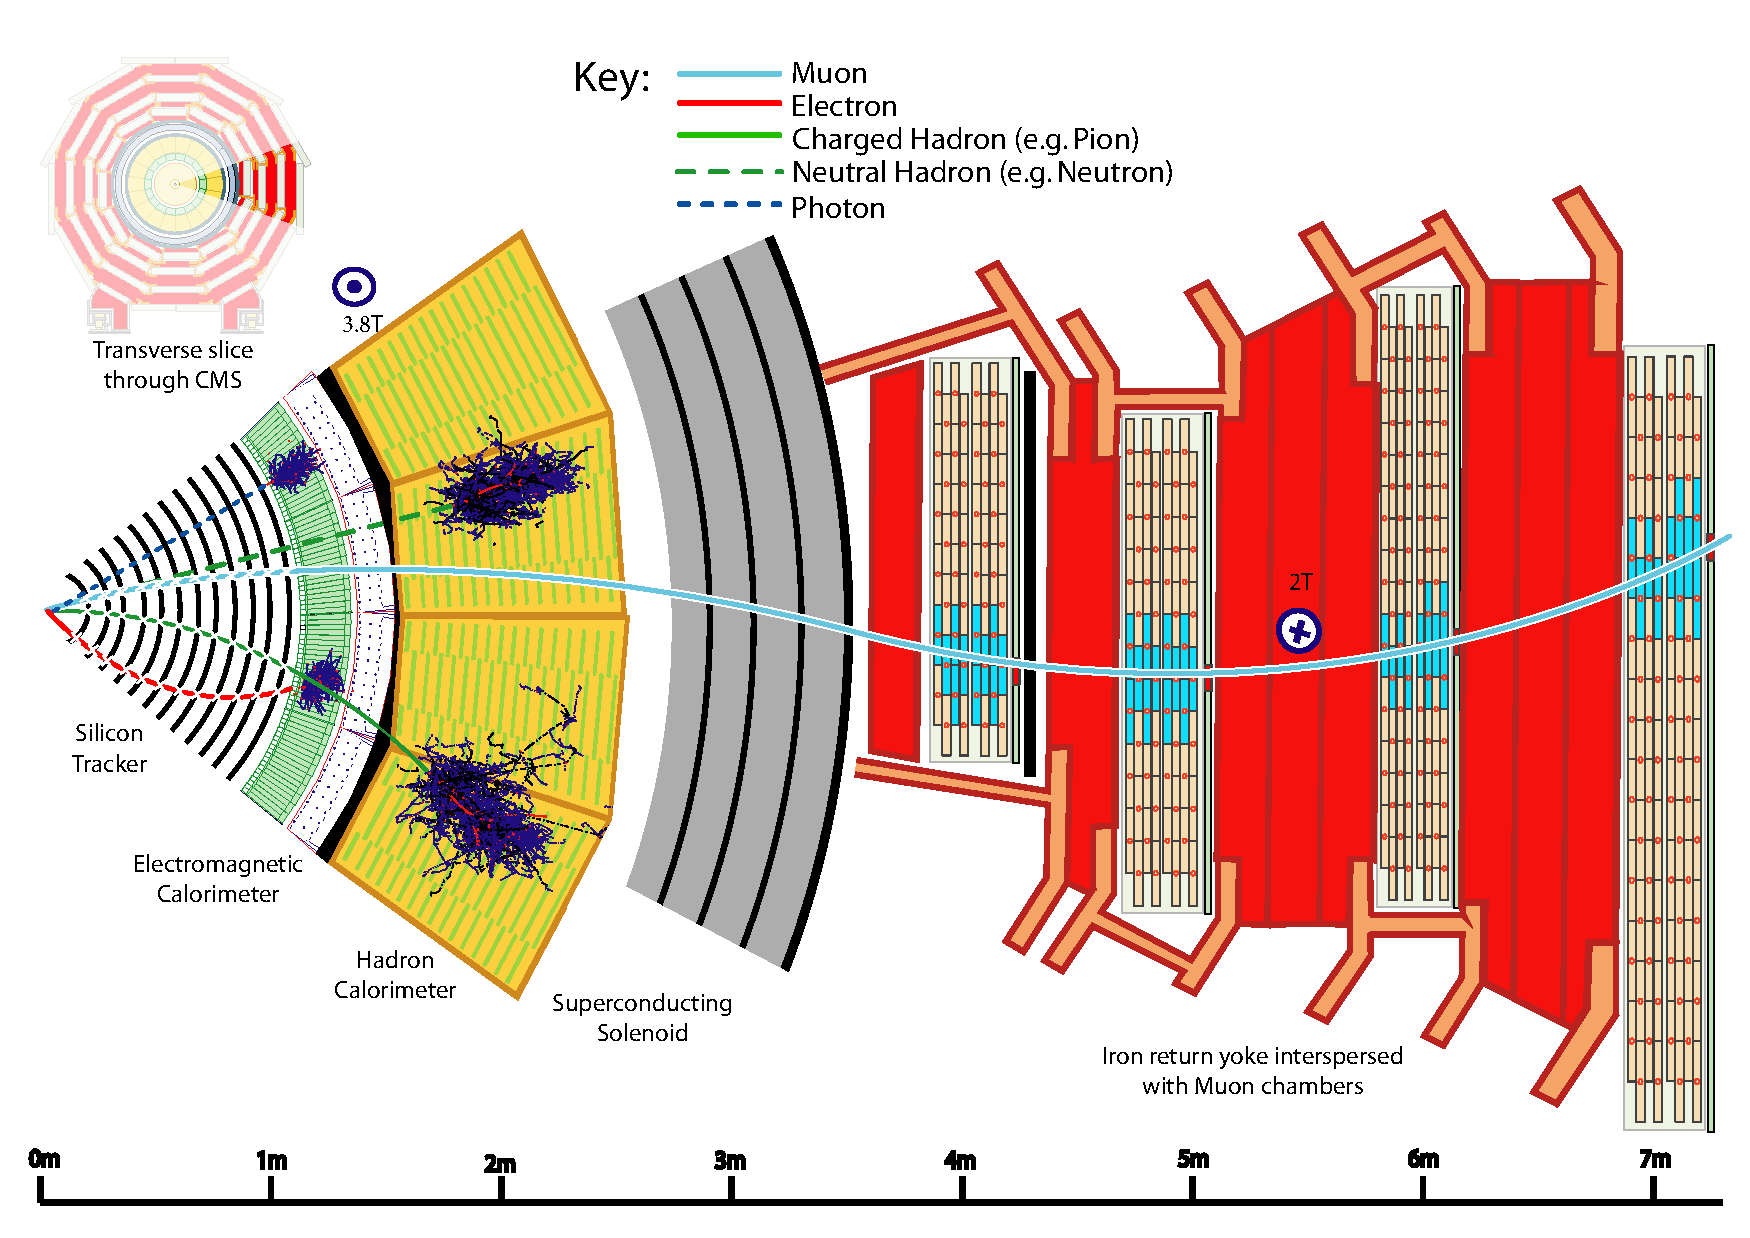
\includegraphics[width=0.75\textwidth]{figures/Transverse_slice_CMS.png}
    \caption[A transverse slice through the CMS detector with the main subsystems and components visible]{A transverse slice through the \acrshort{cms} detector with the main subsystems and components visible (figure obtained from Ref.~\citenum{CMS-PRF-14-001}). Several particles produced at the primary vertex and their interactions with the detector are also depicted.}
    \label{fig:detector_cms_transverse}
\end{figure}

% Maybe mention the upgrades done between Run-1 and Run-2, and possibly even the planned upgrades for Run-3 and Phase-2.
% Phase-1 upgrade TDRs: HCAL \cite{Mans:1481837}, pixels \cite{Dominguez:1481838}, L1T \cite{Tapper:1556311}.
% Phase-2 upgrade TDRs: tracker \cite{Collaboration:2272264}, barrel calorimeters \cite{Collaboration:2283187}, end cap calorimeters \cite{Collaboration:2293646}, muon detectors \cite{Collaboration:2283189}, L1T \cite{Collaboration:2283192}, DAQ \cite{Collaboration:2283193}.
% Can look at CMS detector section in CMS papers for an overview of things. Give more detail where appropriate.


%=========================================================


\subsubsection{Geometry}
\label{subsubsec:geometry}

Collider physics tends to use certain conventions when describing the positions of particles in a detector. The azimuthal angle $\phi$ is the same variable as in cylindrical coordinates, i.e., the angle between the particle's position and the longitudinal axis of the detector (the beam line). Pseudorapidity, denoted by $\eta$, is a coordinate that describes the angle of a particle (after a collision in an accelerator) relative to the beam axis:

\begin{equation}
    \eta = -\ln \left[ \tan \left( \frac{\theta}{2} \right) \right]
    \label{eq:eta_def}
\end{equation}

where $\theta$ is the angle between the particle's three-momentum $\mathbf{p}$ and the positive direction of the beam axis. So as $\theta \rightarrow 0^{\circ}$ (the beam line), $\eta \rightarrow \infty$. Generally, particles with large $\eta$ escape the detector which is why forward calorimeters are in place. The transverse momentum of a particle can be found with $\pt = \lvert \mathbf{p} \rvert / \cosh \eta$.

The subdetectors of \acrshort{cms} are nominally separated into several sections dependent on their geometry, and can mostly be divided into $\eta$ ranges. In the \acrshort{ecal} and \acrshort{hcal}, the barrel region corresponds to $\abseta < \text{1.479}$ and the end cap region $\text{1.479} < \abseta < \text{2.964}$. The \acrshort{hf} occupies $\text{2.964} < \abseta < \text{5.191}$. These boundaries are defined by the edges of the calorimeter towers. The tracker extends out to $\abseta < \text{2.5}$, known as the ``central region''. Its barrel and end cap sections are bound by $\abseta \lesssim \text{1.6}$ and $\text{1.6} \lesssim \abseta \text{2.5}$, respectively. The muon chambers comprise of a central barrel region ($\abseta < \text{1.1}$) and central end cap region ($\text{0.9} \abseta < \text{2.4}$). It overlaps with the barrel since the components are designed parallel and perpendicular to the beam line, not according to $\eta$. The pseudorapidity range of the muon chambers' end cap is restricted compared to the \acrshort{ecal} and \acrshort{hcal} because of the bounds of the tracker, and the steel that surrounds the structure takes up the remainder of the end cap. One quadrant of \acrshort{cms} showing the $\eta$ divisions can be seen in Fig.~\ref{fig:cms_eta_bounds}.

\begin{figure}[htbp]
    \centering
    \includegraphics[width=0.75\textwidth]{figures/cms_eta_ranges.pdf}
    \caption[A quadrant of the CMS detector showing the main subsystems with their radius $R$, longitudinal distance $z$, and pseudorapidity $\eta$ from the interaction point]{A quadrant of the \acrshort{cms} detector showing the main subsystems with their radius $R$, longitudinal distance $z$, and pseudorapidity $\eta$ from the interaction point. The grey box at $3 < \abseta < 5$ and $11 < z < 12$\,m is the hadron forward calorimeter. Figure taken from Ref.~\citenum{cms_dp_end_of_run2}.}
    \label{fig:cms_eta_bounds}
\end{figure}

The distance between two objects can be found with the variable $\Delta R$:

\begin{equation}
\Delta R = \sqrt{(\Delta \eta)^2 + (\Delta \phi)^2}
\label{eq:delta_r}
\end{equation}

It is often used as a distance parameter in jet clustering, or between individual objects in highly-boosted decays.


%=========================================================


\subsection{Data acquisition and triggering}
\label{subsec:cms_recording_data}

With the enormous collision rate at the \acrshort{cms} interaction point, acquiring data requires some thought and ingenuity. Today's electronics cannot handle the bandwidth from recording every single collision, \OrderOf{1 \ \text{petabyte} \ \text{s}^{-1}}. As such, a ``trigger'' is used to select the events that may be of use to analysers. In \acrshort{cms}, a two stage trigger~\cite{Bayatyan:706847} is used: the \acrfull{l1t}, implemented in the detector hardware; and the \acrfull{hlt}~\cite{Cittolin:578006}, a software farm to further reduce the events selected at \acrlong{l1}. The trigger is part of the larger \acrfull{daq} system, an intricate network of custom electronics and commercial processors --- a union of hardware, firmware, and software --- interconnected by multi-gigabit links to record the products of the highest-energy manmade collisions on Earth.


%=========================================================


\subsubsection{The Level-1 Trigger}
\label{subsubsec:detector_l1t}

The \acrlong{l1t} is a set of algorithms (a trigger ``menu'')\footnote{Do I need to say that different menus are used throughout the data-taking periods and for different injectants (heavy ions, etc.)?} implemented in custom hardware designed to reduce the event rate from 40\,MHz to a maximum of 100\,kHz. FPGA and ASIC chips contain the algorithms in firmware, with timing systems synchronised with the \acrshort{lhc} clock. When a collision occurs, particles interact with the detector and registered by the components.

Coarsely-segmented data is sent from the \acrshort{ecal} and \acrshort{hcal} through a two-layer Calorimeter Trigger. These are arrays of custom processors located at Point 5. Layer-1 receives data from the calorimeters over upwards of one thousand fibre optic links, each with multi-gigabit bandwidths. The information from the two subsystems are combined into calorimeter towers, and some simple position- and energy-dependent calibrations are applied.\footnote{Mention something about trigger primitives here?} The data from Layer-1 is then transmitted to Layer-2, again over many high-bandwidth optical links. Here, physics object candidates are identified (\glspl{jet}, \Pe, \Pphoton, \Ptau).\footnote{An overview of the latest Run-2 algorithms for object identification can be found in Ref.~\citenum{Zabi_2017}.} Additional calibrations are applied to them (for example, in Chpt.~\ref{subsec:detector_jecs}), and simple pileup subtraction is performed.\footnote{Do I need to describe in detail how jets are formed? Jet seed, chunky donut PU subtraction, etc... Since it may be relevant for \acrshort{jec}.} Energy sums are also calculated at this stage, such as \etmiss, \HT, and \mht.

In parallel, the various subdetectors in the muon chambers pass information through successive stages, notably the Muon Track-Finder Layer (EXPAND), and is then combined with some of the calorimeter information in a sorting/merging/isolation layer. The output from this layer is combined with the remaining information in Layer-2 in the Global Trigger, a series of \si{\micro}TCA boards with FPGAs. The trigger menu lives here, and all of the information gathered --- object candidates, energy sums, beam conditions --- is provided to it. These triggers may be dependent on the presence a single object or the number of objects of a single class (e.g., one muon, two \glspl{jet}), multiple classes of object (cross triggers), the energy sums, the topologies of objects, and more. The latency given to make a decision on whether to keep or reject an event is 4\,\si{\micro}s.\footnote{Mention pre-scaling of triggers, and that as $\mathcal{L}$ decreases over a fill, the pre-scales change?} A diagram of this data flow is given in Fig.~\ref{fig:cms_l1t_data_flow}.

\begin{figure}[htbp]
    \centering
    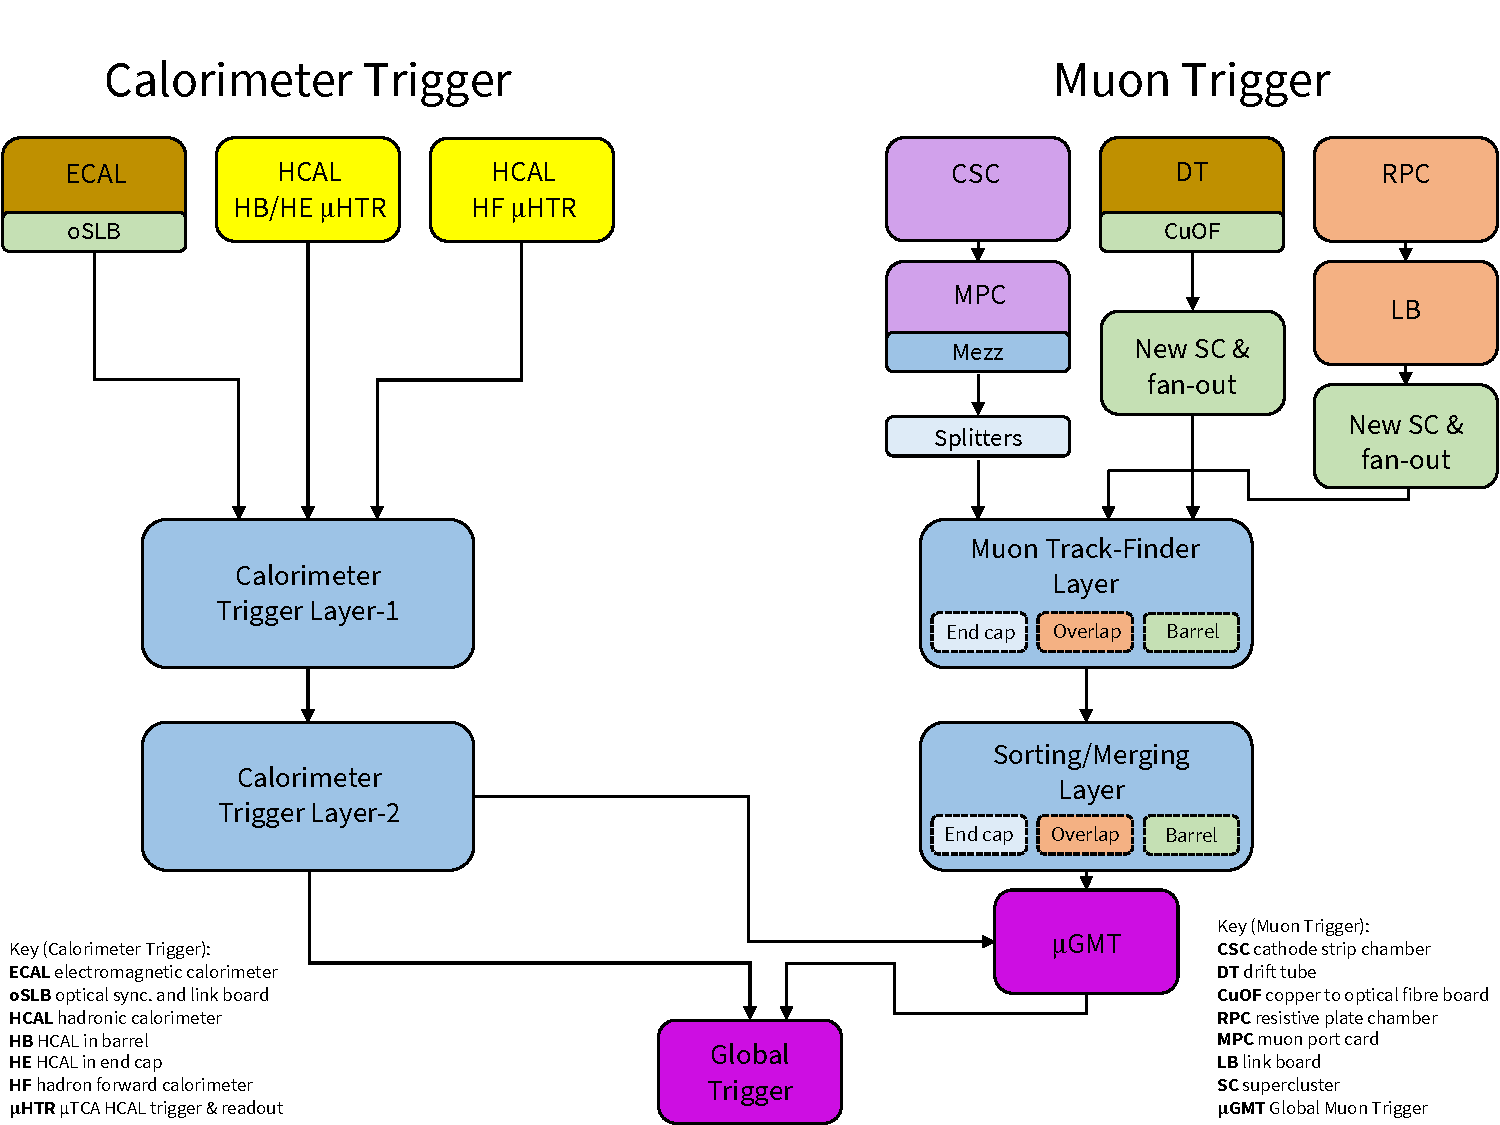
\includegraphics[width=0.75\textwidth]{figures/CMS_L1T_data_flow_key_ordered.pdf}
    \caption[A summary of the CMS Level-1 Trigger data flow from the hits recorded by the subsystems to the Global Trigger]{A summary of the \acrshort{cms} \acrlong{l1t} data flow from the hits recorded by the subsystems to the Global Trigger. Figure reproduced from Ref.~\cite{Dev_2017}.}
    \label{fig:cms_l1t_data_flow}
\end{figure}

A small subset of data from the \acrshort{l1t} is diverted for monitoring purposes. During data taking periods, \acrshort{cms} has a plethora of members that participate in the maintenance and observation of the experiment. At Point 5, shifters monitor the different [areas] collecting information from various sources. Data acquisition, data quality, access to the experimental cavern, the \acrshort{l1t} (which I have performed on numerous occasions), and the \acrshort{hlt} are among them. Experts in these, and more specific, systems are on call on a rotating period. I, myself, have been an on call for Layer-2 of the Calorimeter Trigger several times.

%=========================================================


\subsubsection{The High-Level Trigger}
\label{subsubsec:detector_hlt}

Events that pass a logical \texttt{OR} of the triggers at \acrlong{l1} are transmitted to the \acrshort{hlt}. The higher resolution data collected at the point of collision is available, along with information from the tracker. Populated with Intel Xeon processors (high core count CPUs), approximately 22,000 cores are available (by the end of Run-2) to process the data sent from the \acrshort{l1t}. In order to avoid a back-log, a 100\,kHz input rate allows a \acrshort{hlt} node $\sim$220\,ms to make a decision. High-level software in the \acrshort{cmssw} environment (written in C\texttt{++} and Python, see Chpt.~[REF]) % reference analysis tools/software section
is executed. A larger and more complex trigger menu is available, including the possibility analysis-specific triggers (such as those that target \acrshort{vbf} topologies in Chpt.~\ref{chap:higgstoinv}). Complex variables such as \alphaT can even be calculated and triggered on.

Physics objects are reconstructed further, with algorithms such as \gls{antikt} used to cluster \glspl{jet}~\cite{Cacciari:2008gp}. Additional classification algorithms are also applied to objects, such as the \textsc{DeepCSV} neural network to identify \glspl{bjet}. Some of these algorithms can be computationally expensive. Consequently, approximations/parameterisations are used at \acrshort{hlt} level. A global event reconstruction from the \gls{particleflow} (\acrshort{pf})~\cite{CMS-PAS-PFT-09-001,CMS-PRF-14-001} is performed as well. The [fully-fledged] versions of these kind of algorithms are re-run on the retained events in later stages of postprocessing.

The \acrshort{hlt} reduces the event rate from the maximum 100\,kHz input substantially down to around 1\,kHz. The datastream \OrderOf{\text{6\,GB\,s}^{-1}} is then subject to further processing before the analysts access it. As well as the data being stored on networked hard drives at sites across the globe, back ups are made to magnetic tape for long term storage. As with the \acrlong{l1t}, some data is [diverted] for monitoring, object calibrations, and alignment of detector components.

% CMS Computing TDR: \cite{Bayatyan:838359}.


%=========================================================


\subsection{Simulating CMS data}
\label{subsec:cms_mc}

Data recorded by \acrshort{cms} is paramount for analyses searching for new physics. However, simulated samples are also of high importance. Events for specific processes are generated using \acrfull{mc} random sampling, and the output datasets are often collectively referred to by the method: ``\acrlong{mc}'' or ``\acrshort{mc}''. The datasets are often generated with large numbers of events to minimise the associated statistical uncertainty. \acrshort{mc} samples are useful in a variety of cases: understanding the kinematics of signal processes in searches for new physics, modelling background processes that can mimic signal, and comparisons to data for validation purposes.

A matrix element generator such as \madgraph~\cite{Alwall:2014hca} or \POWHEG~\cite{Nason:2004rx,Frixione:2007vw} models the hard scattering process, usually at \acrfull{lo} but sometimes at higher orders. Events then pass through a hadroniser (usually \PYTHIA~\cite{pythia82} in \acrshort{cms}) to model hadronisation of quarks and gluons, sometimes known as the \emph{parton shower} -- the softer radiation that accompanies the hard scatter. \Glspl{jet} are clustered here by, for example, the \gls{antikt}. The particles are also run through a detector simulation that emulates the configuration and response of the detector in different years. Material interactions and emulation of the triggers are included. \GEANTfour~\cite{AGOSTINELLI2003250,1610988,ALLISON2016186} provides this in \acrshort{cms}. Once the particles have been appropriately simulated, they are given the same postprocessing treatment as actual data, such as executing object tagging algorithms so that the data and simulated samples are as comparable as possible.


%=========================================================


\subsection{Jet energy corrections in the Level-1 Trigger}
\label{subsec:detector_jecs}

Recording the properties of hadrons that are amalgamated into \glspl{jet} is not always consistent across the detector. While the components go through quality control, there is inevitably some variation in their performance. They can degrade at different rates. Some may also receive hits more often than others and be subject to greater radiation damage. As a result, non-uniformity of the detector response --- parameterised in terms of \pt and $\eta$ --- must be compensated for. For \glspl{jet}, this comes in the form of \gls{jec}.

As outlined in Chpt.~\ref{subsubsec:detector_l1t}, the trigger primitives from the \acrshort{ecal} and \acrshort{hcal} enter Layer-1 of the Calorimeter Trigger and coarse position- and energy-dependent calibrations are applied. \glspl{jet} as objects are initially identified in Layer-2, and preliminary calibrations correct their energy. Disregarding these, even at this early stage in the data acquisition workflow, can affect the efficiency and rate of the \acrlong{l1t}. It is therefore important to re-derive the calibrations regularly, since the configuration of the detector and beam conditions change over the lifetime of the experiment.

When a new round of calibrations are derived, there are many steps before this one. Preceding it, Layer-1 experts calculate their scale factors for the calorimeter towers. Once performed, the \acrlong{jec} are then derived in \acrshort{cmssw}.


%=========================================================


\subsubsection{The procedure}
\label{subsubsec:detector_jec_procedure}

\acrshort{qcd} multijet \acrshort{mc} datasets with a large \pt range used to derive the Layer-1 and Layer-2 calibrations. Corresponding \glspl{jet} in data for this process are often mismeasured (so providing good calibrations in the most difficult scenario is a good test), and \acrshort{mc} events contain ``truth-level'' information from the generator. Ntuples are made from these which have the Layer-1 corrections applied. Referring to the processing chain in Chpt.~\ref{subsec:cms_mc}, the jets these calibrations are derived for are post-hadronisation, but before interaction with the detector. They will be referred to as ``\acrfull{l1} jets''. The reference jets directly from the generator (``GenJets'' as colloquialised in \acrshort{cms}) are important for matching to our \acrshort{l1} jets to ensure we are not mistakenly using jets [birthed] in the parton shower that have no reference point.

The reference and \acrshort{l1} jets are matched using the variable $\Delta R$ (see Eq.~\ref{eq:delta_r}). The algorithm used to match the jets does so by inspecting each \acrshort{l1} jet in descending \pt and searching for a reference jet with $\Delta R < 0.25$. If there is more than one match, the reference jet with the smallest $\Delta R$ is taken. Then the next \acrshort{l1} jet (and so on) follows the same procedure, with the previous reference jet removed from the matching collection.

The pairs of jets are categorised into sixteen bins of \abseta, the highest granularity available since the calibrations must run quickly on hardware. Each in is then analysed in turn.

Within each \abseta bin, the jet pairs are subdivided into bins of the transverse momentum of the reference jet (\ptRef). The bin widths, like \abseta, are variable. The ratio of the transverse momentum of the \acrshort{l1} jet (\ptLOne) to \ptRef is taken for each pair of jets. Our metric for measuring the detector response is the mean of these ratios:

\begin{equation}
    r_j = \langle \ptLOne / \ptRef \rangle
    \label{eq:jec_detector_response}
\end{equation}

The reciprocal of the $r_j$ vs. \ptLOne is inspected and a correction curve is fitted. A gaussian captures the peak at low \pt and the following equation\footnote{Go into more detail regarding the equation? Reasoning, etc.} is used for the tail:

\begin{equation}
    \ptsup{{\mathrm{L1, \ corr.}}} = \ptLOne \cdot \left( p_0 + \frac{p_1}{ \left(\log_{10} \ptLOne \right) ^2 + p_2 } + p_3 \cdot \exp \left( -p_4 \left( \log_{10} \ptLOne - p_5 \right)^2 \right) \right)
    \label{eq:corr_curve_jec_tail}
\end{equation}

The input parameters for the function may not be adequate, so they are tuned to capture the low-\pt spike and high-\pt plateau (see Fig.~\ref{fig:detector_jecs_corr_curves} for a visual representation). The value of this fit function in each \ptRef bin is exported.

\begin{figure}[htbp]
    \centering
    \begin{subfigure}[b]{0.45\textwidth}
        \includegraphics[width=\textwidth]{./figures/jecs/corrCurveBarrel.pdf}
        \caption{$0.435 < \abseta < 0.783$ (Barrel)}
        \label{fig:detector_jecs_corr_curve_Barrel}
    \end{subfigure}
    \hfill
    \begin{subfigure}[b]{0.45\textwidth}
        \includegraphics[width=\textwidth]{./figures/jecs/corrCurveHF.pdf}
        \caption{$4.191 < \abseta < 5.191$ (HF)}
        \label{fig:detector_jecs_corr_curve_HF}
    \end{subfigure}
\caption[Examples of correction curves used to calibrate the jet energies in two \abseta bins]{Examples of correction curves used to calibrate the jet energies in two \abseta bins. The reciprocal of the response is plotted against the \pt of the \acrlong{l1} jet, and a complex function (Eq.~\ref{eq:jec_detector_response}) fits the points. These plots are from the jet energy corrections performed on 2018 \acrshort{qcd} \acrlong{mc}.}
\label{fig:detector_jecs_corr_curves}
\end{figure}

Once all \abseta bins have been inspected, the calibrations are consolidated in several forms. A machine-readable lookup table is [put] in the firmware of the Layer-2 hardware, so that the corrections are applied in the trigger. A version is added to the \acrlong{l1t} packages in \acrshort{cmssw} so that the next steps in the calibration chain can utilise them.

A closure test is conducted to validate the corrections we have just produced. The \acrshort{mc} ntuples are regenerated with the \acrshort{jec} applied. Jet matching is performed and the calibrations are checked. Many diagnostic and performance plots are produced to ensure the calibrations are [performing] as expected. These can be inclusive of the number of pileup interactions, or split into ranges to see if the calibrations differ between them. Examples of these are Fig.~\ref{fig:detector_jecs_scatter_BE} showing scatter plots of \ptRef vs. \ptLOne before and after \acrshort{jec} are applied, and Fig.~\ref{fig:detector_jecs_response} shows the response.

% Taken directly from second year report.
% Tidy up and improve, describing the whole workflow, at least briefly (uses QCD multijet MC, send through detector sim with expected detector layout/response(?), corrections made as function of pt and eta (mention the 16 eta bins), then closure tests - regenerate MC with corrections and check they're applied correctly, make plots, circulate corrections in various formats).
% Can also look in Section 20 of my lab book for more info. Can pull material from the trigger/DPG presentations I've given (I should have the actual pdf/png plots in Service Work - Jet Energy Corrections in the Level-1 Trigger/)
% Link the repository somewhere: https://github.com/eshwen/L1JetEnergyCorrections. Stress that I only forked it from the original developers and made modifications on top of it
% Should I note the pt values and abseta bins for the calibrations?

\begin{figure}[htbp]
    \centering
    \begin{subfigure}[b]{0.45\textwidth}
        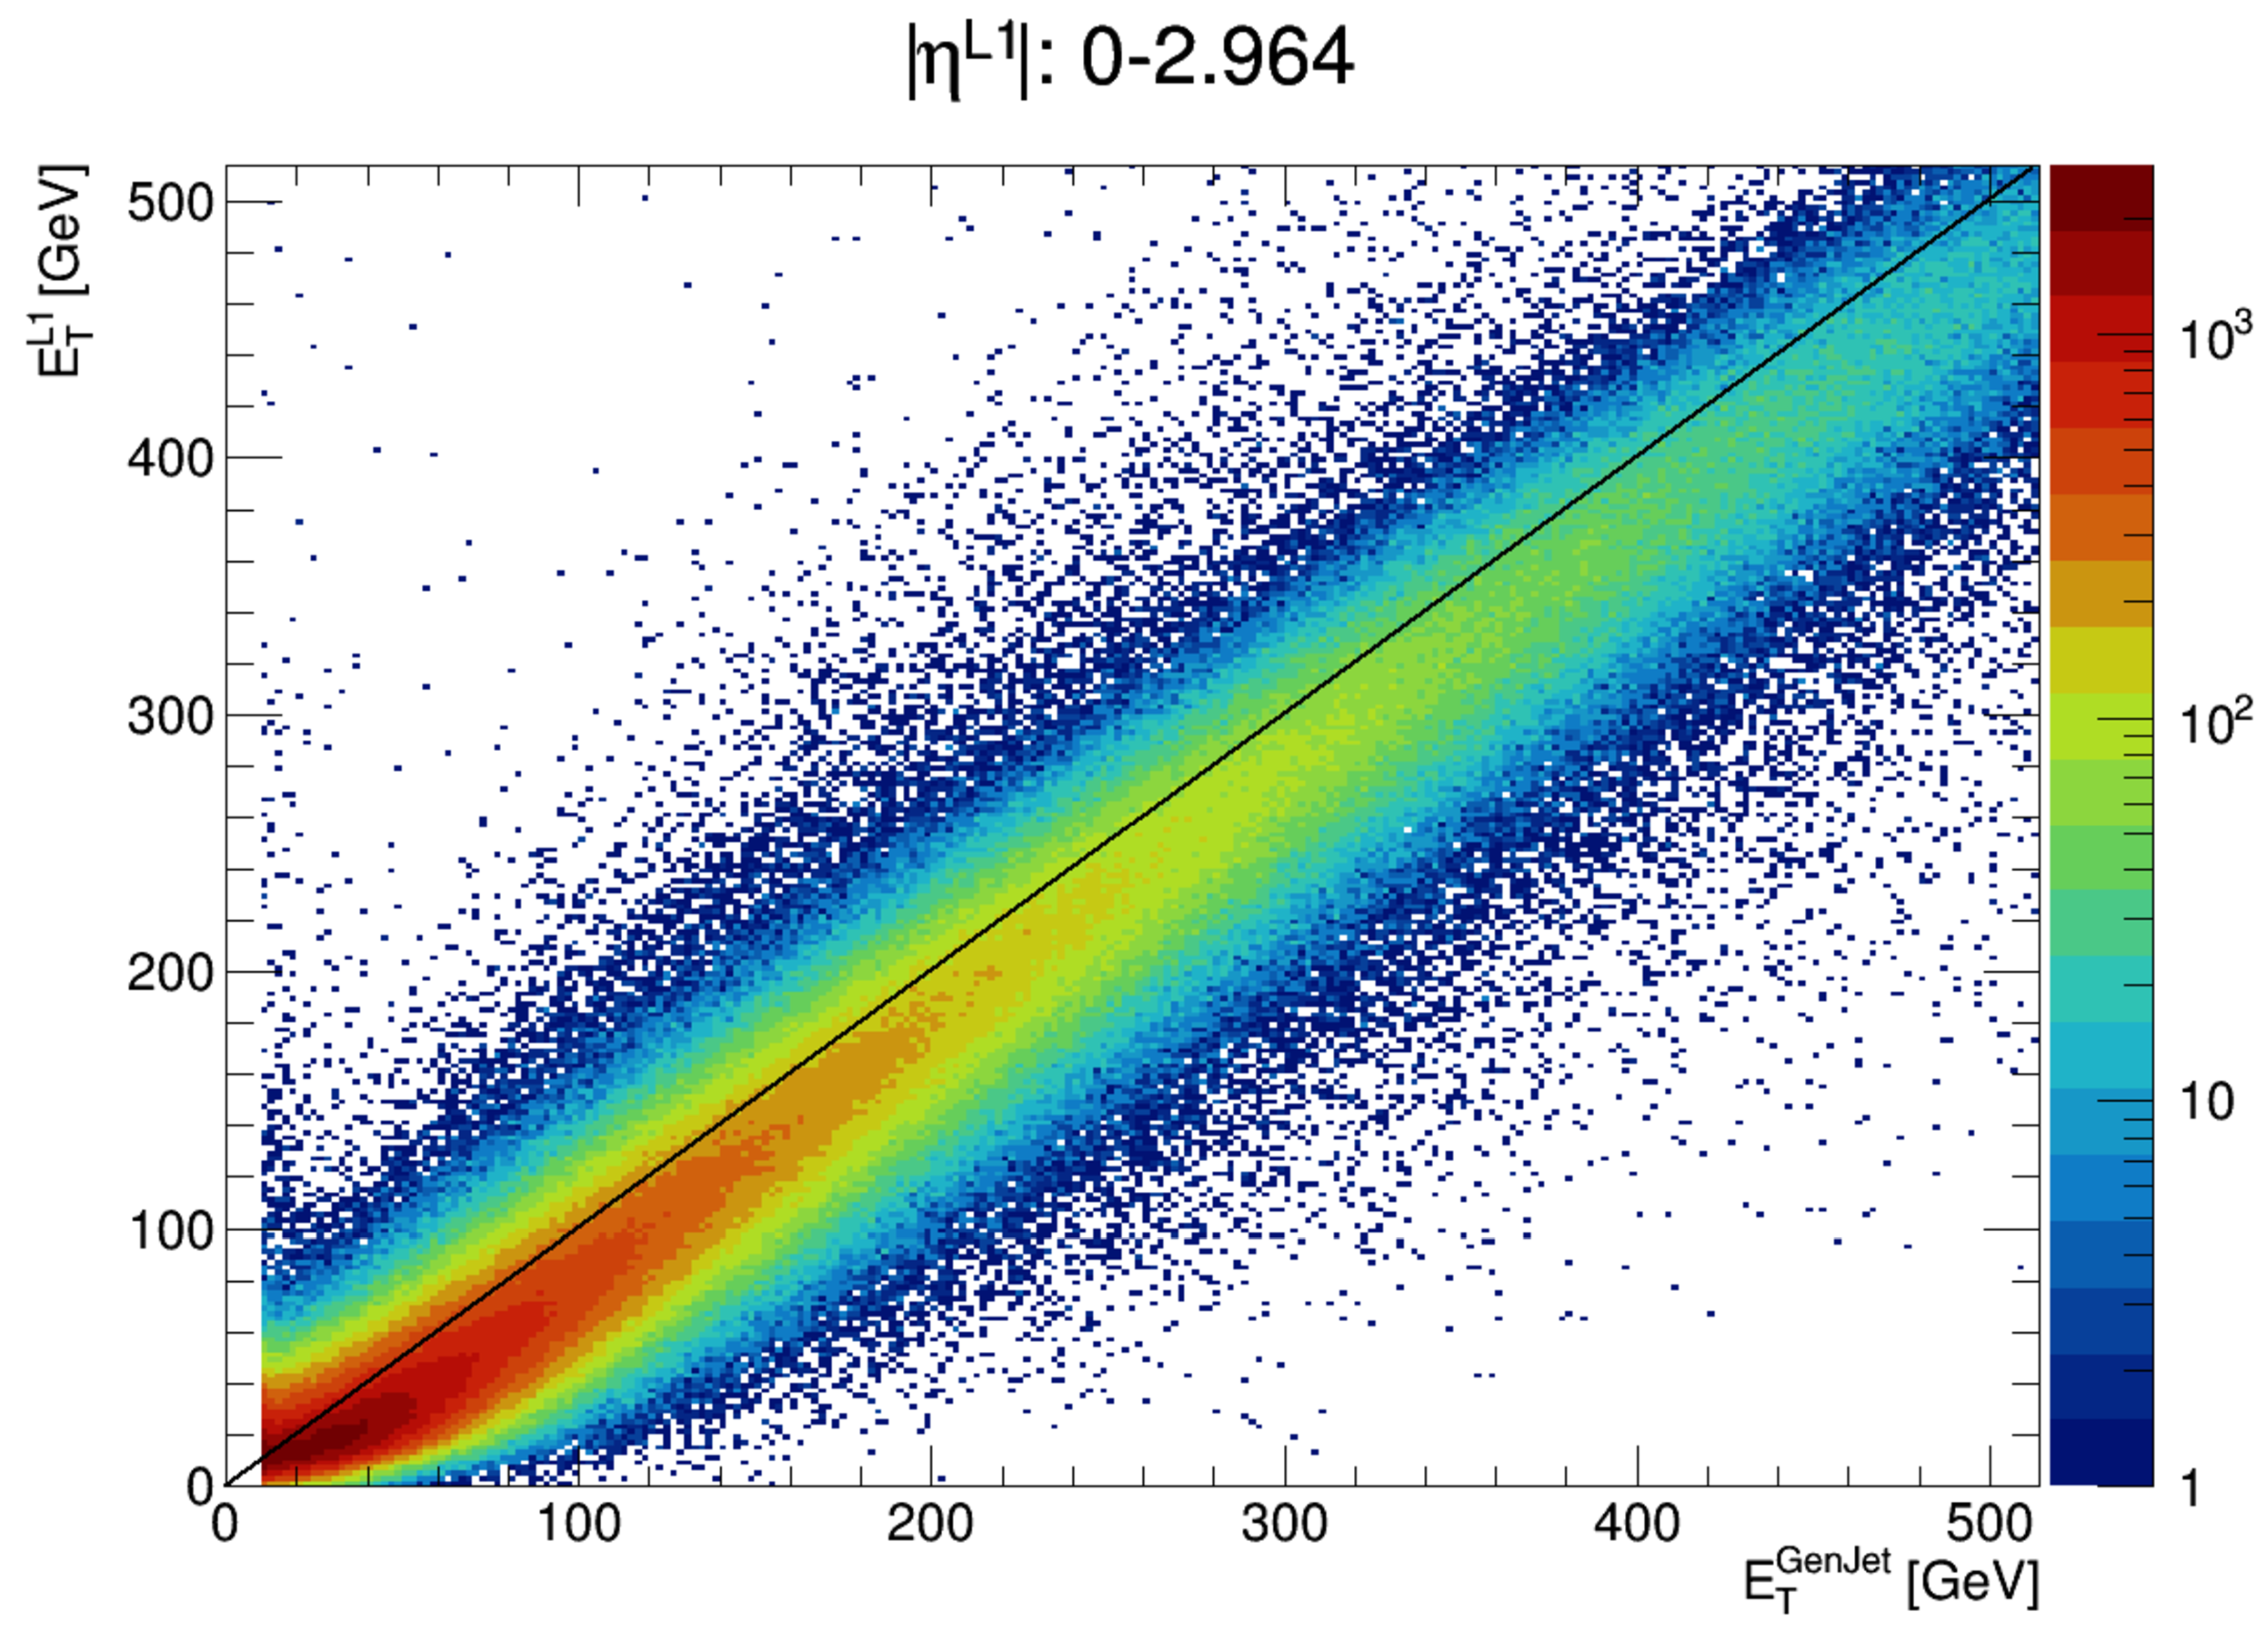
\includegraphics[width=\textwidth]{./figures/jecs/scatterPlotBeforeBE.png}
        \caption{Before corrections}
        \label{fig:detector_jecs_scatter_before_BE}
    \end{subfigure}
    \hfill
    \begin{subfigure}[b]{0.45\textwidth}
        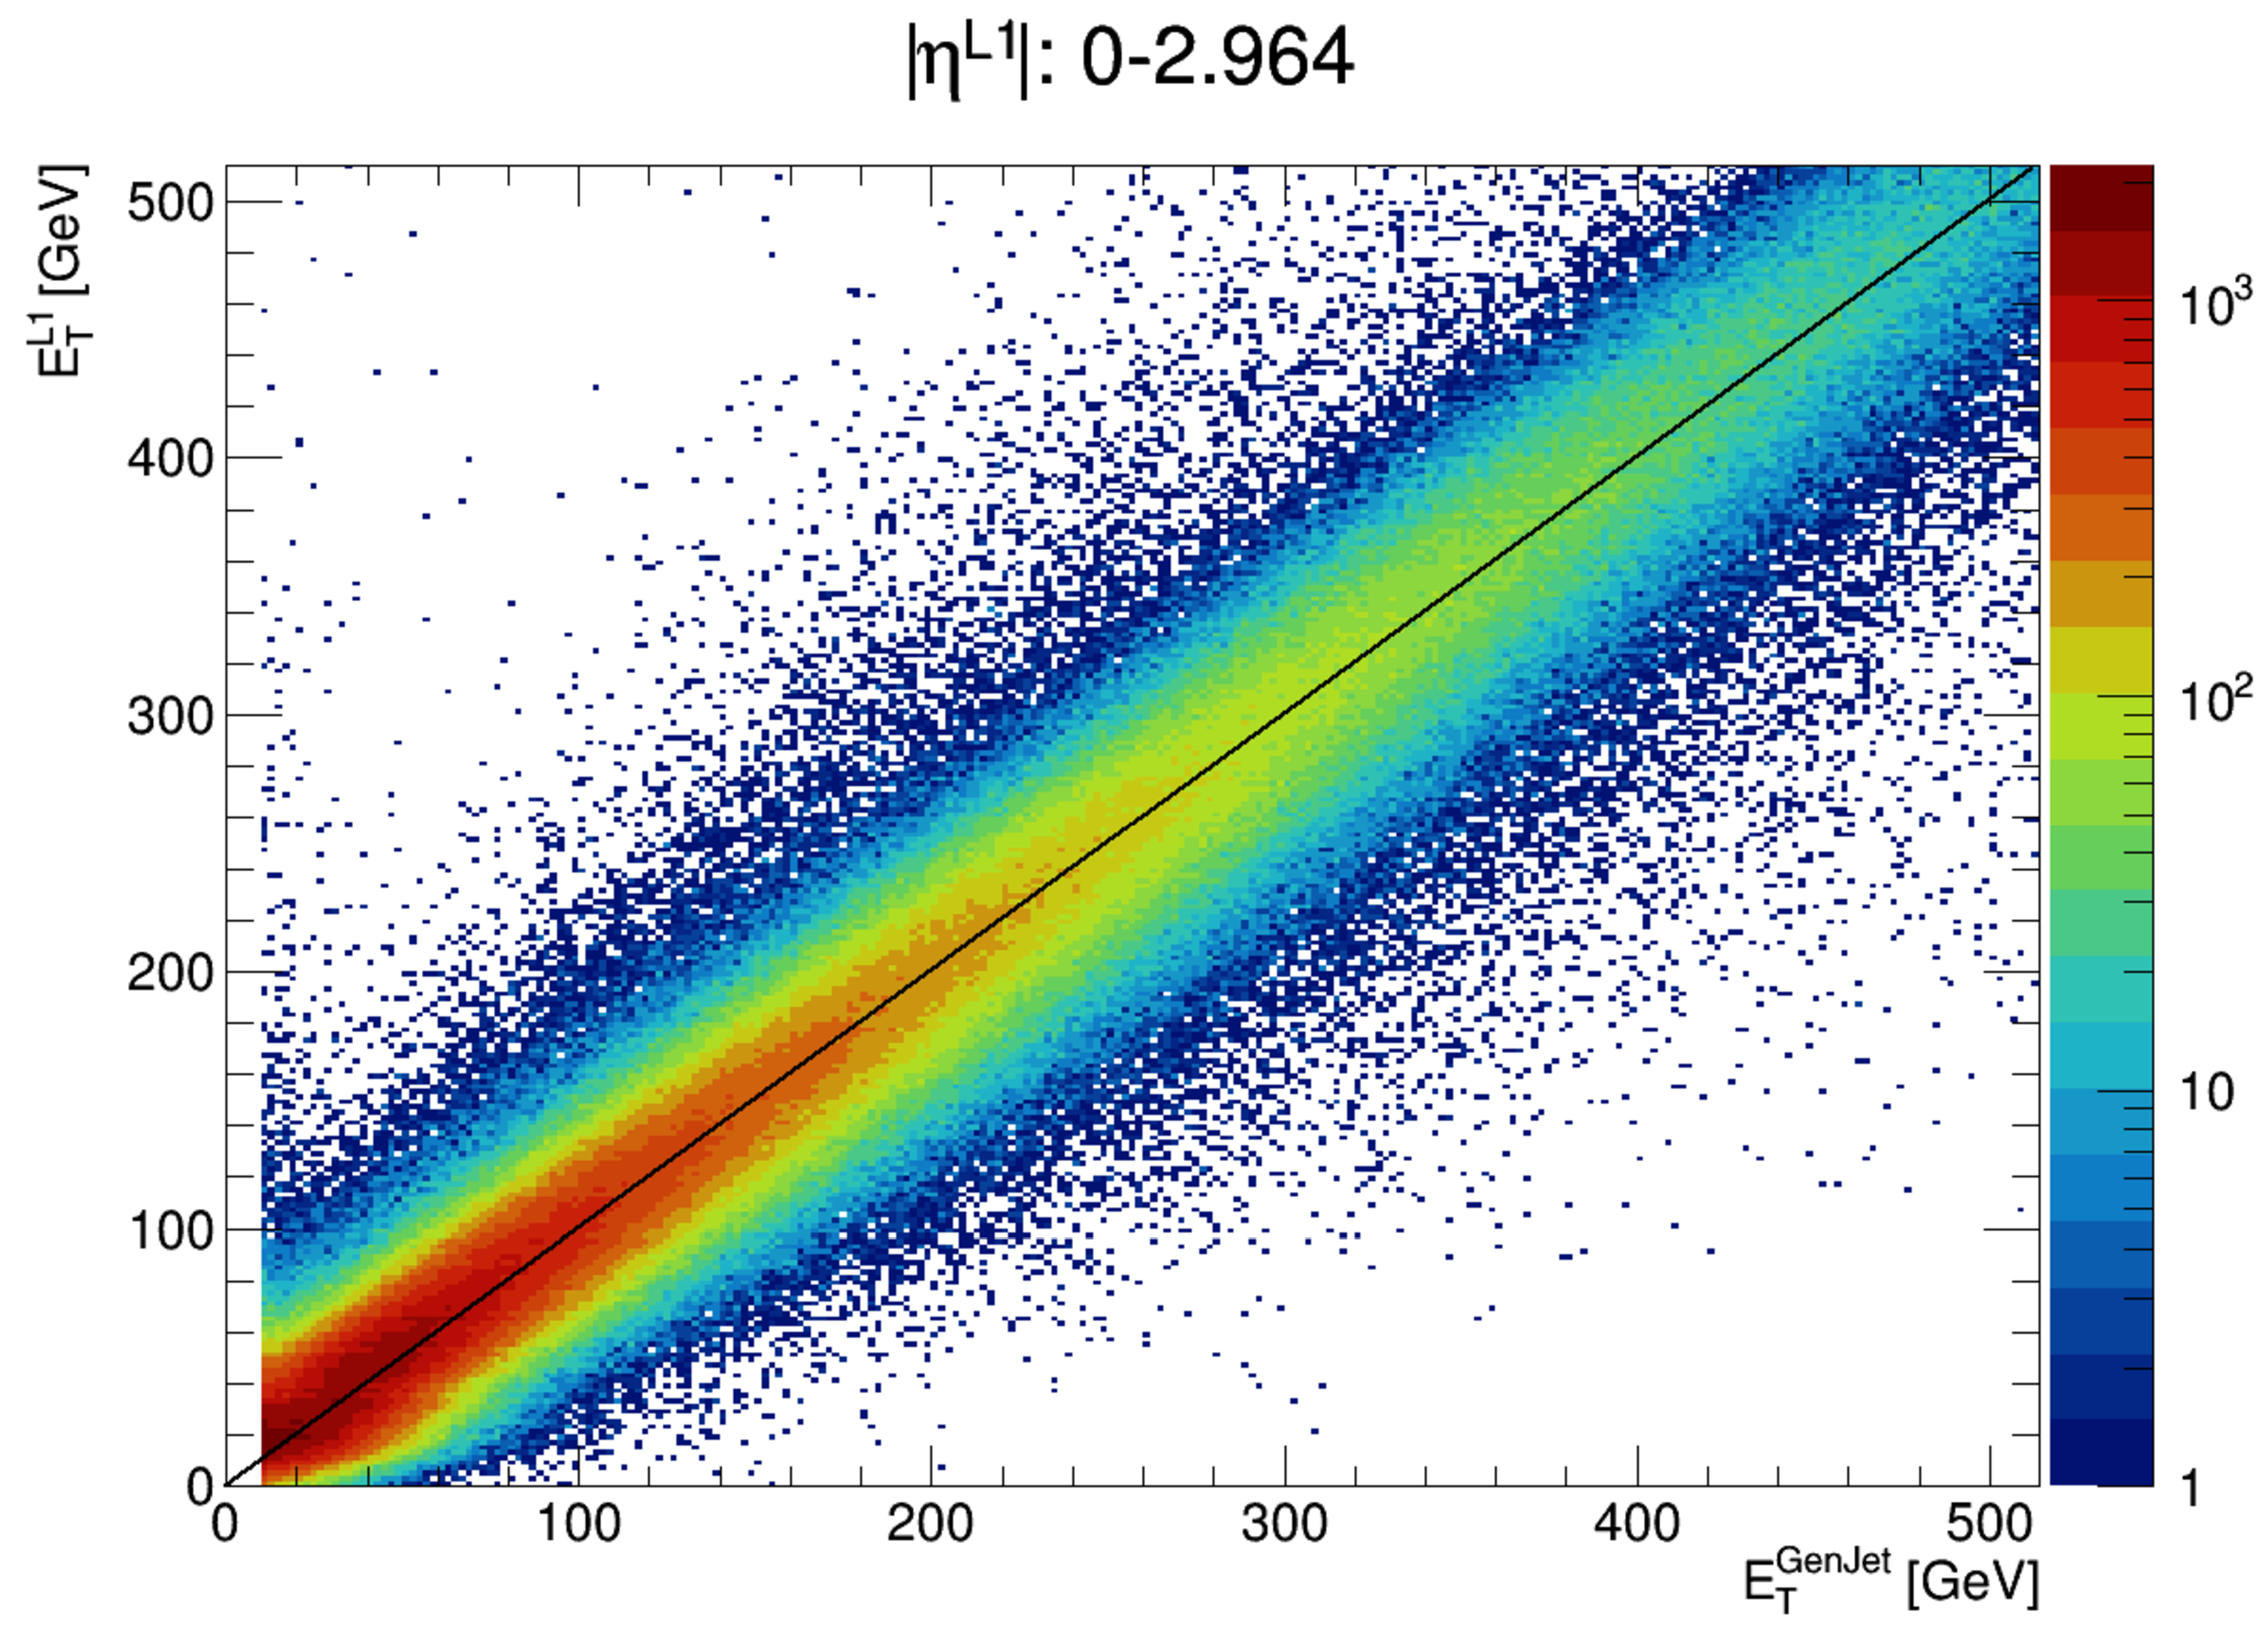
\includegraphics[width=\textwidth]{./figures/jecs/scatterPlotAfterBE.png}
        \caption{After corrections}
        \label{fig:detector_jecs_scatter_after_BE}
    \end{subfigure}
\caption[The energies of matched pairs of jets in the entire barrel and end cap, in the pileup 40--50 range, before and after jet energy corrections have been applied]{The energies of matched pairs of jets in the entire barrel and end cap, in the pileup 40--50 range, before and after \acrlong{jec} have been applied. After calibrations, the distribution is much more symmetrical. An equivalent plot using \glspl{jet} from \acrshort{lhc} data is expected to look similar after applying these calibrations.}
\label{fig:detector_jecs_scatter_BE}
\end{figure}

\begin{figure}[htbp]
    \centering
    \begin{subfigure}[b]{0.45\textwidth}
        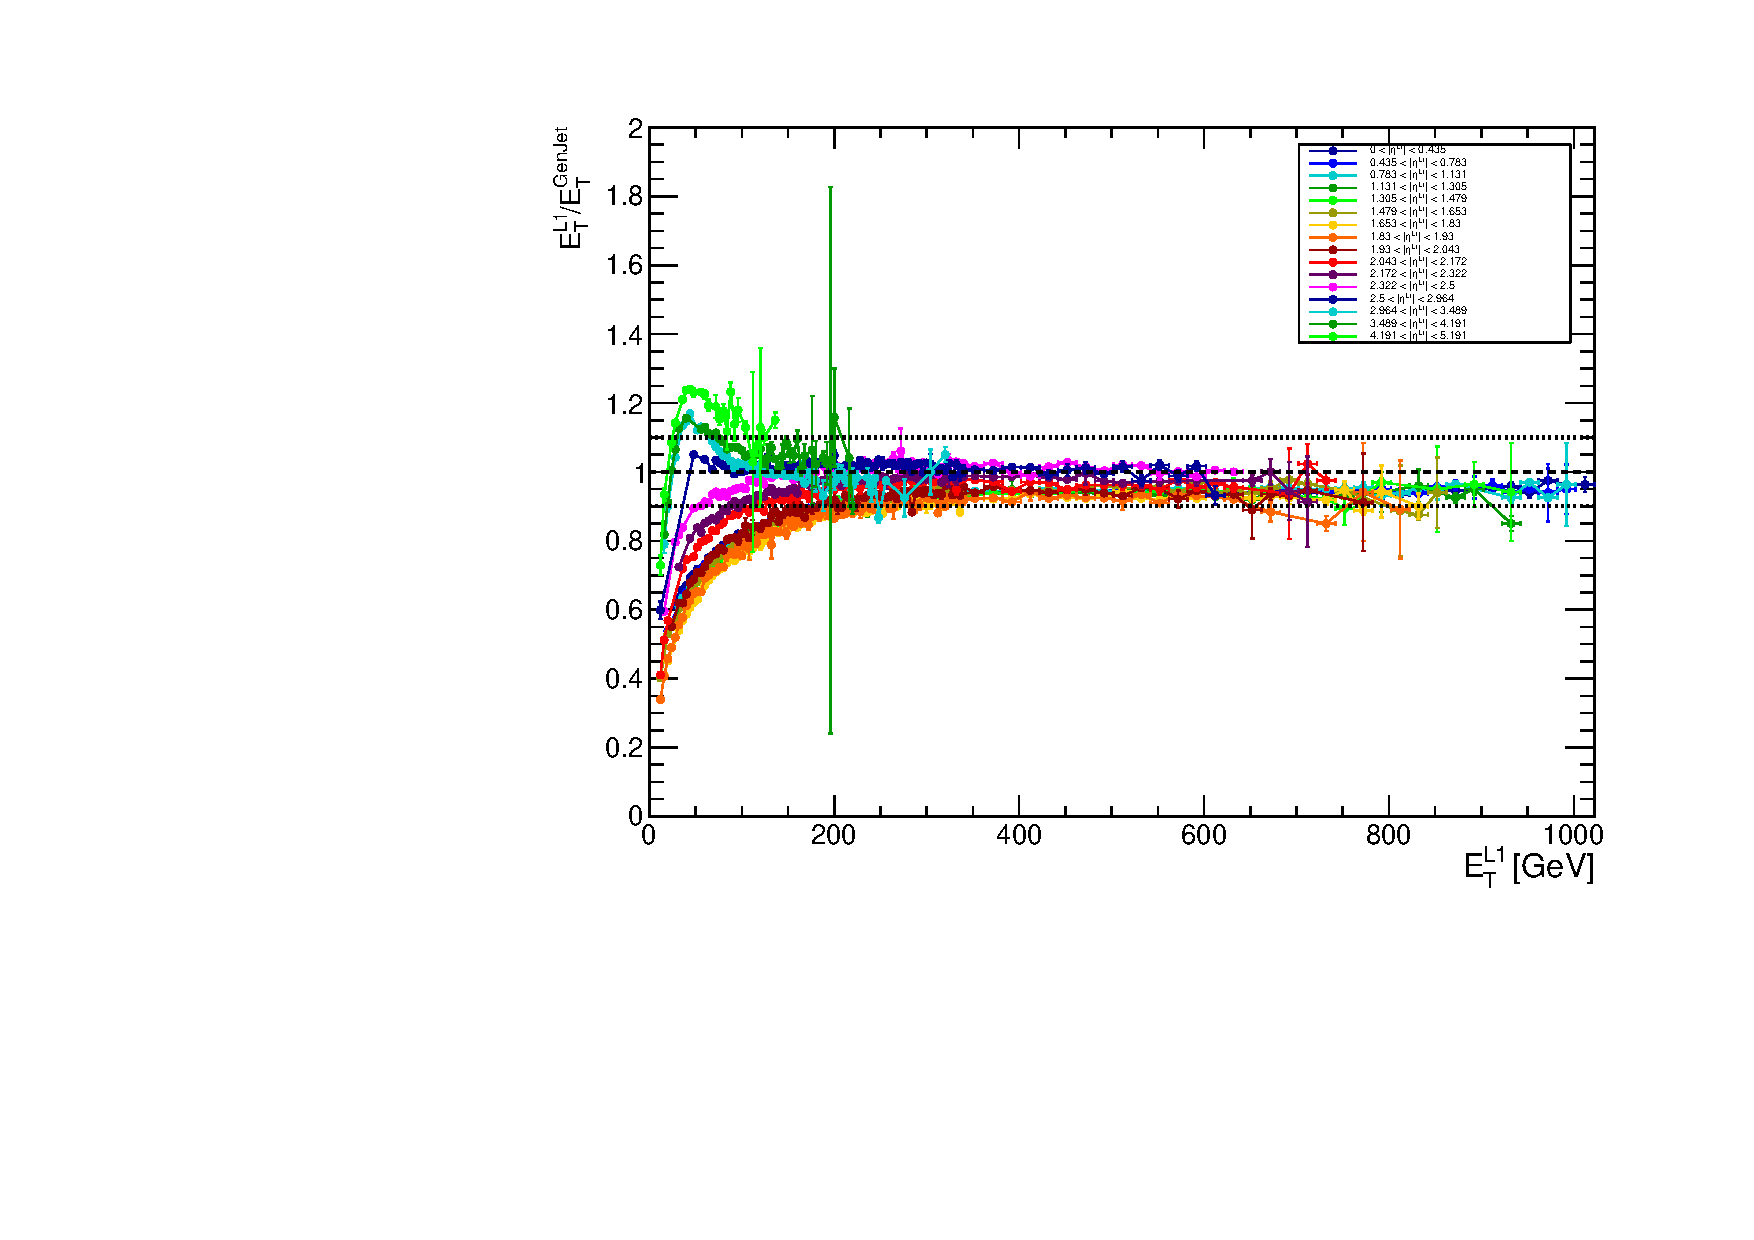
\includegraphics[width=\textwidth]{./figures/jecs/response_before.pdf}
        \caption{Before corrections}
        \label{fig:detector_jecs_response_before}
    \end{subfigure}
    \hfill
    \begin{subfigure}[b]{0.45\textwidth}
        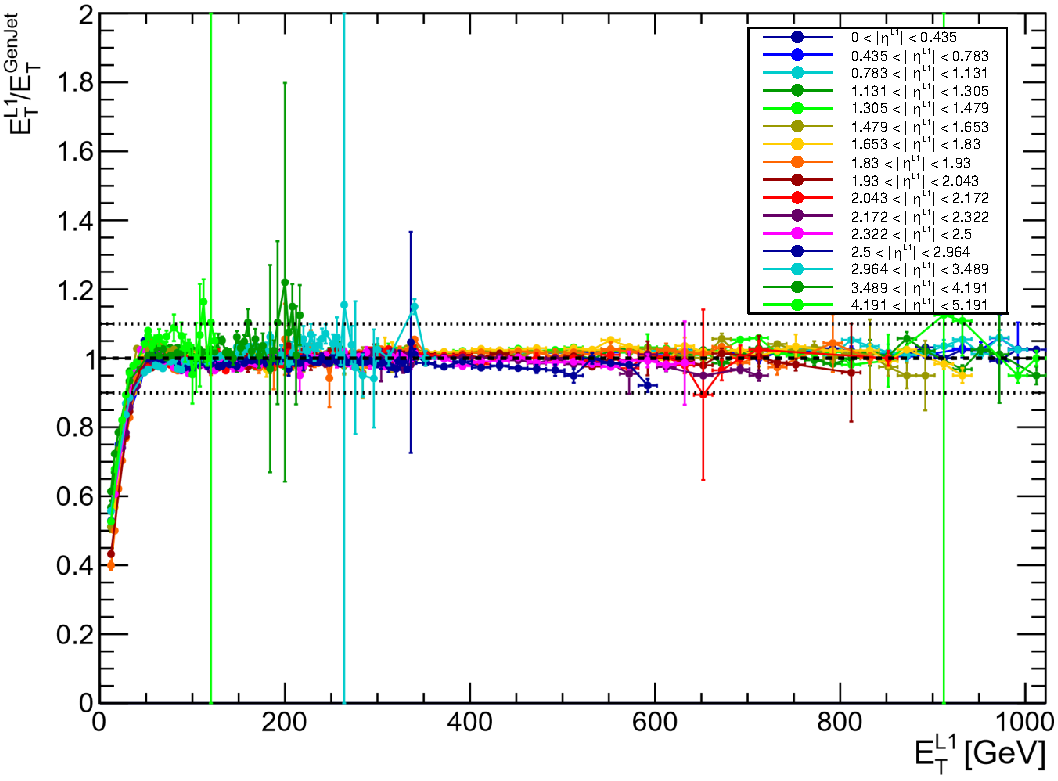
\includegraphics[width=\textwidth]{./figures/jecs/response_after.pdf}
        \caption{After corrections}
        \label{fig:detector_jecs_response_after}
    \end{subfigure}
\caption[The response curves in each \abseta bin as a function of \ptLOne, in the pileup 40--50 range, before and after jet energy corrections are applied]{The response curves in each \abseta bin as a function of \ptLOne, in the pileup 40--50 range, before and after \gls{jec} are applied. Note that in panel b, the $x$-axis is the corrected \ptLOne.}
\label{fig:detector_jecs_response}
\end{figure}

%=========================================================
